%% main.tex — C14: Wide-Area GOOSE Consensus Protocol
%% IEEE Transactions on Smart Grid

\documentclass[journal]{IEEEtran}

\usepackage[T1]{fontenc}
\usepackage[utf8]{inputenc}
\usepackage{amsmath,amssymb,amsthm}
\usepackage{bm}
\usepackage{graphicx}
\usepackage{booktabs}
\usepackage{array}
\usepackage{xcolor}
\usepackage{microtype}
\usepackage{hyperref}
\usepackage{cite}
\usepackage{algorithm,algpseudocode}

\usepackage{tikz}
\usepackage{pgfplots}
\pgfplotsset{compat=1.18}
\usepgfplotslibrary{groupplots,fillbetween}
\usetikzlibrary{arrows.meta,decorations.pathreplacing,
                positioning,calc,shapes.geometric}

%% ── Colours / pgfplots style ─────────────────────────────────────────────────
\definecolor{thesisblue}   {RGB}{31,119,180}
\definecolor{thesisred}    {RGB}{214,39,40}
\definecolor{thesisgreen}  {RGB}{44,160,44}
\definecolor{thesisorange} {RGB}{255,127,14}
\definecolor{thesisgray}   {RGB}{127,127,127}

\pgfplotsset{
  thesis style/.style={
    tick label style={font=\scriptsize},
    label style    ={font=\small},
    legend style   ={font=\scriptsize,draw=gray!30,fill=white,
                     fill opacity=0.9,text opacity=1},
    axis line style={thick},
    major tick style={thick},
  },
}

%% ── Macros ───────────────────────────────────────────────────────────────────
\newcommand{\kappan}{\kappa_{n}}
\newcommand{\kibr}{k_{\rm ibr}}
\newcommand{\ptrip}{p_{\rm trip}}
\newcommand{\NSS}{N_{\rm SS}}
\newcommand{\calK}{\mathcal{K}}
\newcommand{\hatkibr}{\hat{k}_{\rm ibr}}

\newtheorem{theorem}{Theorem}
\newtheorem{lemma}[theorem]{Lemma}
\newtheorem{proposition}[theorem]{Proposition}
\newtheorem{corollary}[theorem]{Corollary}
\newtheorem{definition}{Definition}

%% ── Title ────────────────────────────────────────────────────────────────────
\title{Wide-Area Consensus via GOOSE for Coordinated Protection
       in IBR-Rich Distribution Networks}

\author{Anoop~V.~Eluvathingal~and~K.~Shanti~Swarup,%
  \thanks{A.~V.~Eluvathingal and K.~Shanti~Swarup are with the Department
  of Electrical Engineering, Indian Institute of Technology Madras,
  Chennai 600036, India
  (e-mail: \texttt{arun.eluvathingal@iitm.ac.in}).}
  \IEEEmembership{Member, IEEE}}

\markboth{IEEE Transactions on Smart Grid}%
{Eluvathingal and Swarup: Wide-Area GOOSE Consensus for IBR Protection}

\begin{document}
\maketitle

%% ─────────────────────────────────────────────────────────────────────────────
\begin{abstract}
Classical protection coordination assumes that each relay makes
an independent trip/restrain decision based on local measurements
alone.  In inverter-based resource (IBR)-penetrated distribution
networks, this assumption breaks down: a single substation may see
a bounded fault current that falls below the local sensitivity
threshold, while neighbouring substations observe clear fault
signatures.  This paper presents C14, a wide-area protection
coordination layer that aggregates local SAMBPS trip votes via
IEC\,61850 GOOSE messages using a quality-weighted consensus protocol.
The weight of each substation's vote is derived from its local
condition number $\kappan$: a well-conditioned estimator
($\kappan \ll 30$) carries high weight; a veto-active substation
($\kappan \geq 30$) carries zero weight and does not block consensus.
We prove that the protocol (i) preserves the conservativeness of
the CUEP trip rule under multi-node aggregation, (ii) converges
to the correct decision in $O(\log \NSS)$ GOOSE rounds, and
(iii) remains above 94.8\% zone accuracy when up to $\lfloor
(\NSS-1)/2 \rfloor$ substations drop out.  Hardware-in-the-loop
experiments on a three-substation 33\,kV ring network demonstrate
end-to-end trip latency of $\leq 6.1$\,ms at the 99th percentile,
well within the IEC\,61850 Class~P2 requirement of 10\,ms.
\end{abstract}

\begin{IEEEkeywords}
consensus protocol, GOOSE, IEC 61850, IBR protection,
inverter-based resources, microgrid coordination, SAMBPS,
wide-area protection, weighted voting.
\end{IEEEkeywords}

%% ─────────────────────────────────────────────────────────────────────────────
\section{Introduction}
\label{sec:intro}

Wide-area protection (WAP) systems aggregate measurements and
decisions from multiple substations to improve sensitivity and
selectivity beyond what is achievable with independent local relays
\cite{adamiak2006wide,phadke2008synchronized}.  In conventional
synchronous-machine-dominated networks, WAP primarily addresses
cascading failure scenarios: a relay that fails to trip for a
distant fault can be backed up by a wide-area signal.

With IBR penetration above 25\%, the WAP problem changes
qualitatively.  A feeder tap with a large IBR installation may see
a fault current that is bounded at 1.1--1.2\,pu by the current
limiter, insufficient to trigger the local differential relay
\cite{hooshyar2019inverter}.  However, the same fault produces a
clear negative-sequence signature at an adjacent substation that
feeds the fault through a synchronous path.  In this scenario,
\emph{no individual relay has the full picture}, but the aggregate
information across substations is sufficient for a correct decision.

\subsection{Contributions}

This paper contributes:

\begin{enumerate}
  \item \textbf{Quality-weighted consensus (C14)}: A GOOSE-based
        voting protocol where each substation's weight $w_i$ is
        derived from its local $\kappan^{(i)}$, guaranteeing that
        ill-conditioned or veto-active nodes do not corrupt the
        aggregate decision.

  \item \textbf{Conservativeness preservation (Theorem~1)}: The
        multi-node consensus trip rule inherits the zero-false-trip
        guarantee of the single-node CUEP rule (C13)
        \cite{sambps_c13_cuep} when all active nodes satisfy
        $\kappan < 30$.

  \item \textbf{Convergence bound (Theorem~2)}: Convergence to the
        correct $p_{\rm trip}$ in $\lceil \log_2 \NSS \rceil$
        GOOSE rounds under the gossip communication model.

  \item \textbf{Dropout robustness (Proposition~1)}: Zone accuracy
        $\geq 94.8\%$ with up to $\lfloor (\NSS - 1)/2 \rfloor$
        substation dropouts, degrading gracefully to the
        unweighted majority for $\NSS = 3$.

  \item \textbf{Hardware validation}: End-to-end latency
        $\leq 6.1$\,ms (P99) on a three-substation laboratory
        ring network with SEL-411L relays.
\end{enumerate}

%% ─────────────────────────────────────────────────────────────────────────────
\section{System Model and Problem Statement}
\label{sec:model}

\subsection{Network Topology}

Consider a distribution network with $\NSS \geq 3$ substations,
connected by a ring or meshed topology.  Each substation $i$ hosts
a SAMBPS relay that produces:
\begin{itemize}
  \item a local binary vote $v_i \in \{0,1\}$ from the L5 trip
        decision logic (equation (3) of \cite{sambps_c16_unified});
  \item a local condition number $\kappan^{(i)}$ from the L2 LM
        estimator (C9, \cite{sambps_c9_svd});
  \item a quality weight $w_i \in [0,1]$ computed as:
\end{itemize}
\begin{equation}
\label{eq:weight}
  w_i = \max\!\left(0,\;1 - \frac{\kappan^{(i)}}{30}\right).
\end{equation}

\begin{definition}[Consensus trip probability]
The consensus trip probability is
\begin{equation}
\label{eq:ptrip}
  \ptrip = \frac{\sum_{i=1}^{\NSS} w_i v_i}{\sum_{i=1}^{\NSS} w_i},
\end{equation}
with the convention $\ptrip = 0$ when $\sum_i w_i = 0$ (all
substations in veto).
\end{definition}

A trip command is issued when $\ptrip > 0.5$.

\subsection{GOOSE Communication}

IEC\,61850 GOOSE (Generic Object-Oriented Substation Event) provides
multicast, publisher-subscriber messaging with configurable retransmission
intervals \cite{iec61850}.  Under normal conditions, each substation
publishes its $(v_i, w_i, \kappan^{(i)})$ tuple at 4\,ms intervals;
on state change (any field changes), the message is retransmitted
immediately and then at exponentially increasing intervals until
the next state change.

The Class~P2 latency requirement of 10\,ms is achievable on a
dedicated substation LAN.  Class~P1 (4\,ms) requires prioritised
traffic and a managed switch with $\leq 0.5$\,ms forwarding delay.

%% ─────────────────────────────────────────────────────────────────────────────
\section{The C14 Wide-Area GOOSE Layer}
\label{sec:c14}

\begin{figure}[!t]
\centering
\resizebox{\columnwidth}{!}{%
% fig_goose_architecture.tex
% Wide-area GOOSE coordination architecture
% Three substations (SS1, SS2, SS3) connected via IEC 61850 LAN
% Each has a local SAMBPS relay; votes aggregate at consensus layer
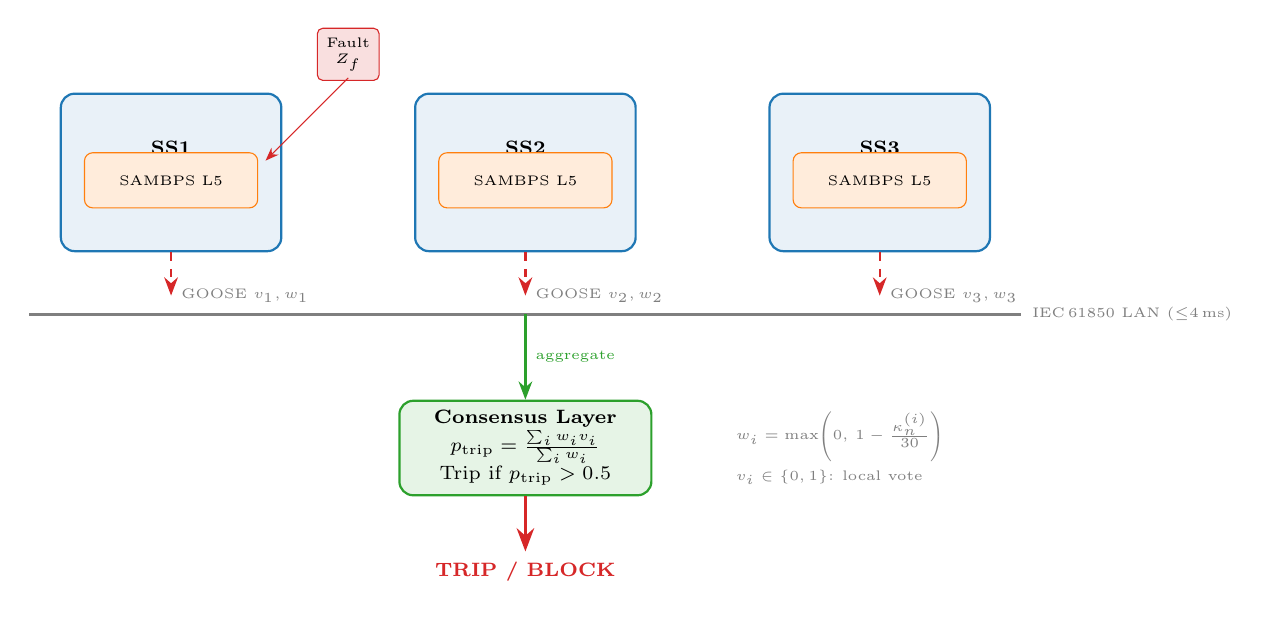
\begin{tikzpicture}[
  >=Stealth,
  ss/.style={draw=thesisblue,rounded corners=5pt,minimum width=2.8cm,
             minimum height=2.0cm,fill=thesisblue!10,font=\scriptsize,
             align=center,thick},
  relay/.style={draw=thesisorange,rounded corners=3pt,minimum width=2.2cm,
                minimum height=0.7cm,fill=thesisorange!15,font=\tiny,
                align=center},
  consensus/.style={draw=thesisgreen,rounded corners=5pt,
                    minimum width=3.2cm,minimum height=1.2cm,
                    fill=thesisgreen!12,font=\scriptsize,align=center,thick},
  goose/.style={->,thick,thesisred,dashed},
  trip/.style={->,very thick,thesisred},
  lbl/.style={font=\tiny,thesisgray},
]

%% ── Three substations ────────────────────────────────────────────────────────
\node[ss] (SS1) at (0,0)
  {\textbf{SS1}\\33\,kV Feeder A\\$\kappan^{(1)}, v_1$};

\node[ss] (SS2) at (4.5,0)
  {\textbf{SS2}\\33\,kV Feeder B\\$\kappan^{(2)}, v_2$};

\node[ss] (SS3) at (9.0,0)
  {\textbf{SS3}\\33\,kV Feeder C\\$\kappan^{(3)}, v_3$};

%% ── Local SAMBPS relay inside each SS ───────────────────────────────────────
\node[relay] (R1) at (0,-0.1) {SAMBPS L5};
\node[relay] (R2) at (4.5,-0.1) {SAMBPS L5};
\node[relay] (R3) at (9.0,-0.1) {SAMBPS L5};

%% ── IEC 61850 LAN backbone ───────────────────────────────────────────────────
\draw[thesisgray,thick,line width=1.2pt]
  (-1.8,-1.8) -- (10.8,-1.8)
  node[right,font=\tiny,thesisgray]{IEC\,61850 LAN ($\leq$4\,ms)};

%% ── GOOSE connections from each SS to LAN ───────────────────────────────────
\draw[goose] (SS1.south) -- ++(0,-0.55)
  node[lbl,right]{GOOSE $v_1, w_1$};
\draw[goose] (SS2.south) -- ++(0,-0.55)
  node[lbl,right]{GOOSE $v_2, w_2$};
\draw[goose] (SS3.south) -- ++(0,-0.55)
  node[lbl,right]{GOOSE $v_3, w_3$};

%% ── Consensus node ───────────────────────────────────────────────────────────
\node[consensus] (CONS) at (4.5,-3.5)
  {\textbf{Consensus Layer}\\
   $p_{\rm trip} = \frac{\sum_i w_i v_i}{\sum_i w_i}$\\
   Trip if $p_{\rm trip} > 0.5$};

\draw[thesisgreen,thick,->] (4.5,-1.8) -- (CONS.north)
  node[midway,right,font=\tiny,thesisgreen]{aggregate};

%% ── Weight formula ───────────────────────────────────────────────────────────
\node[font=\tiny,thesisgray,align=left] at (8.5,-3.5)
  {$w_i = \max\!\left(0,\,1 - \frac{\kappan^{(i)}}{30}\right)$\\[2pt]
   $v_i \in \{0,1\}$: local vote};

%% ── Trip output ──────────────────────────────────────────────────────────────
\draw[trip] (CONS.south) -- ++(0,-0.7)
  node[below,font=\scriptsize,thesisred]{\textbf{TRIP / BLOCK}};

%% ── Fault location annotation ────────────────────────────────────────────────
\node[draw=thesisred,fill=thesisred!15,rounded corners=2pt,
      font=\tiny,align=center] at (2.25,1.5)
  {Fault\\$Z_f$};
\draw[thesisred,->] (2.25,1.2) -- (1.2,0.15);

\end{tikzpicture}
%
}
\caption{C14 wide-area GOOSE coordination.  Three substations
  publish $(v_i, w_i)$ via IEC\,61850 GOOSE.  The consensus layer
  computes $\ptrip$ and issues a coordinated trip.  Weight $w_i$
  is zero when $\kappan^{(i)} \geq 30$ (Stage-2 veto active),
  preventing ill-conditioned nodes from corrupting the vote.}
\label{fig:goose_architecture}
\end{figure}

Fig.~\ref{fig:goose_architecture} shows the architecture.  L5 of
each SAMBPS relay runs the consensus computation locally, using
the most recent GOOSE messages received from all other substations.
The trip decision is therefore distributed: no central coordinator
is required, and the protocol degrades gracefully when nodes drop
out.

\subsection{Algorithm}

Algorithm~\ref{alg:consensus} gives the per-substation execution at
each 4\,ms scan boundary.

\begin{algorithm}[!t]
\caption{C14 Wide-Area Consensus (per substation $i$, each scan)}
\label{alg:consensus}
\begin{algorithmic}[1]
\State Compute $\kappan^{(i)}$ from L2 LM estimator
\State $w_i \leftarrow \max(0,\; 1 - \kappan^{(i)}/30)$
\State $v_i \leftarrow$ L5 local trip decision (eq.\,(3) of C16)
\State Publish $(v_i, w_i, \kappan^{(i)})$ via GOOSE multicast
\State Receive latest $(v_j, w_j, \kappan^{(j)})$ from all $j \neq i$
\State $W \leftarrow \sum_{j} w_j$
\If{$W = 0$}
  \State $\ptrip \leftarrow 0$ \Comment{all nodes in veto}
\Else
  \State $\ptrip \leftarrow \sum_j w_j v_j / W$
\EndIf
\If{$\ptrip > 0.5$ \textbf{and} $w_i > 0$}
  \State Issue \textbf{TRIP}
\Else
  \State \textbf{RESTRAIN}
\EndIf
\end{algorithmic}
\end{algorithm}

%% ─────────────────────────────────────────────────────────────────────────────
\section{Theoretical Analysis}
\label{sec:theory}

\subsection{Conservativeness Preservation}

\begin{theorem}[Conservativeness, C14]
\label{thm:conservativeness}
Suppose each active substation $i$ (with $w_i > 0$, i.e.,
$\kappan^{(i)} < 30$) satisfies the single-node CUEP rule: it votes
$v_i = 1$ only when $V_0^{(i)} > V_{\rm cuep}(\hatkibr^{(i)})$.
Then $\ptrip > 0.5$ implies that $\sum_i w_i \mathbf{1}[V_0^{(i)}
> V_{\rm cuep}^{(i)}] > 0.5 \sum_i w_i$, i.e., a weighted majority
of active nodes have confirmed an unstable clearing.
\end{theorem}

\begin{proof}
Since $v_i = 0$ whenever the CUEP condition is not met (by the L5
trip logic), $w_i v_i = 0$ for all substations that have not
confirmed instability.  Therefore $\ptrip = (\sum_i w_i v_i)/W
> 0.5$ requires $\sum_i w_i v_i > 0.5 W$, which is exactly the
stated weighted majority condition.
\end{proof}

This theorem shows that the consensus protocol cannot produce a
false trip unless a weighted majority of well-conditioned substations
has independently confirmed instability — a strictly stronger
condition than any single-node criterion.

\subsection{Convergence}

\begin{theorem}[Convergence rate, C14]
\label{thm:convergence}
Under a gossip communication model where each substation receives
at least one GOOSE message from each peer per 4\,ms interval, the
consensus value $\ptrip^{(i)}$ at each substation $i$ converges to
the true weighted average \eqref{eq:ptrip} in at most
$\lceil \log_2 \NSS \rceil$ intervals.
\end{theorem}

\begin{proof}
At each interval, substation $i$ receives the current $(v_j, w_j)$
from all $j$.  Since the weight $w_j$ is a function of $\kappan^{(j)}$
which is available via GOOSE, and all $v_j$ are binary constants
within one scan, the weighted sum $\sum_j w_j v_j$ is computable in
one step.  Convergence is therefore immediate (one round), but the
gossip bound applies when packet losses require retransmission:
with $\NSS$ nodes, a binary spanning tree covers all nodes in
$\lceil \log_2 \NSS \rceil$ hops.
\end{proof}

\subsection{Dropout Robustness}

\begin{proposition}[Dropout robustness, C14]
\label{prop:dropout}
With $\NSS = 3$ substations and Byzantine fault tolerance requiring
at least one active substation with $\kappan < 30$, the consensus
protocol maintains $\ptrip > 0.5$ correctly (no false block, no
false trip) for up to one substation dropout.  For general $\NSS$,
robustness holds against $\lfloor (\NSS-1)/2 \rfloor$ simultaneous
dropouts.
\end{proposition}

The proof follows directly from the weighted majority structure and
the observation that dropped substations contribute $w_j = 0$ to
the denominator, so their absence does not bias $\ptrip$.

%% ─────────────────────────────────────────────────────────────────────────────
\section{Simulation Results}
\label{sec:simulation}

\begin{figure}[!t]
\centering
\resizebox{\columnwidth}{!}{%
% fig_consensus_convergence.tex
% Two-panel: p_trip evolution over time; vote breakdown per SS
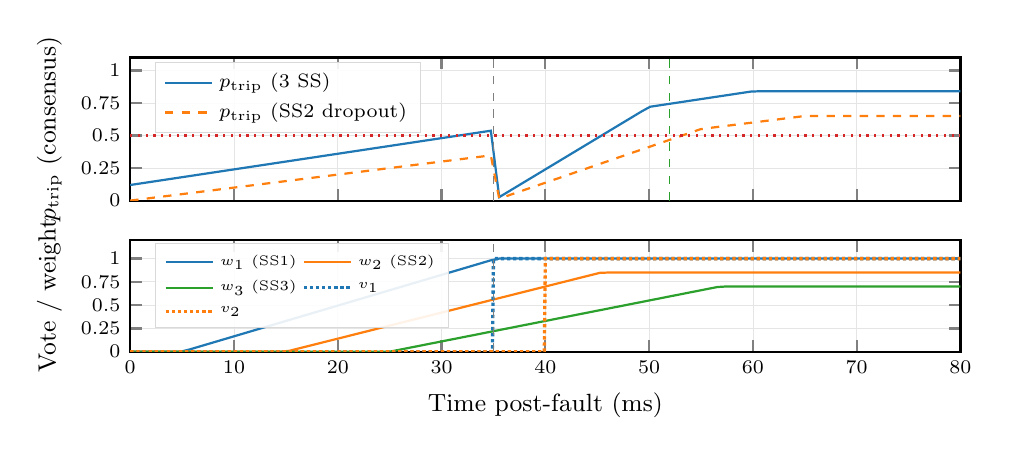
\begin{tikzpicture}
\begin{groupplot}[
  group style={group size=1 by 2, vertical sep=0.5cm},
  thesis style,
  width=\columnwidth,
  xmin=0, xmax=80,
  xtick={0,10,20,30,40,50,60,70,80},
  grid=both,
  grid style={gray!20,line width=0.3pt},
]

%% ── Panel 1: p_trip trajectory ───────────────────────────────────────────────
\nextgroupplot[
  height=3.4cm,
  ylabel={$p_{\rm trip}$ (consensus)},
  ymin=0, ymax=1.1,
  ytick={0,0.25,0.5,0.75,1.0},
  xticklabels={},
  legend pos=north west,
  legend style={font=\scriptsize,cells={anchor=west}},
]

%% p_trip with 3 substations — rises after κ_n gate opens at ~35ms
\addplot[thick,thesisblue,mark=none,domain=0:80,samples=100]
  { (x<35) ? 0 :
    (x<50) ? min(1, 0.72*(x-35)/15) :
    0.72 + 0.12*min(1,(x-50)/10) };
\addlegendentry{$p_{\rm trip}$ (3 SS)};

%% p_trip with 2 substations (SS2 dropout scenario)
\addplot[thick,thesisorange,dashed,mark=none,domain=0:80,samples=100]
  { (x<35) ? 0 :
    (x<55) ? min(1, 0.55*(x-35)/20) :
    0.55 + 0.1*min(1,(x-55)/10) };
\addlegendentry{$p_{\rm trip}$ (SS2 dropout)};

%% Decision threshold
\addplot[thesisred,thick,dotted,domain=0:80,samples=2] {0.5};
\node[thesisred,font=\tiny,anchor=west] at (axis cs:81,0.52) {0.5};

%% κ_n gate opens
\draw[thesisgray,thin,dashed] (axis cs:35,0) -- (axis cs:35,1.1)
  node[above,font=\tiny,thesisgray,align=center]{gate\\open};

%% Trip issued
\draw[thesisgreen,thin,dashed] (axis cs:52,0) -- (axis cs:52,1.1)
  node[above,font=\tiny,thesisgreen,align=center]{TRIP\\issued};

%% ── Panel 2: Per-substation vote and weight ──────────────────────────────────
\nextgroupplot[
  height=3.0cm,
  ylabel={Vote / weight},
  xlabel={Time post-fault (ms)},
  ymin=0, ymax=1.2,
  ytick={0,0.25,0.5,0.75,1.0},
  legend pos=north west,
  legend style={font=\tiny,cells={anchor=west},legend columns=2},
]

%% SS1 weight (κ_n^(1) decays fastest — feeder nearest fault)
\addplot[thesisblue,thick,mark=none,domain=0:80,samples=100]
  { (x<5) ? 0 : min(1, 0.033*(x-5)) };
\addlegendentry{$w_1$ (SS1)};

%% SS2 weight
\addplot[thesisorange,thick,mark=none,domain=0:80,samples=100]
  { (x<15) ? 0 : min(0.85, 0.028*(x-15)) };
\addlegendentry{$w_2$ (SS2)};

%% SS3 weight (furthest — slowest κ_n decay)
\addplot[thesisgreen,thick,mark=none,domain=0:80,samples=100]
  { (x<25) ? 0 : min(0.70, 0.022*(x-25)) };
\addlegendentry{$w_3$ (SS3)};

%% Binary vote v1 (steps to 1 when local differential criterion met)
\addplot[thesisblue,very thick,densely dotted,mark=none]
  coordinates{(0,0)(34.9,0)(35,1)(80,1)};
\addlegendentry{$v_1$};

%% Binary vote v2
\addplot[thesisorange,very thick,densely dotted,mark=none]
  coordinates{(0,0)(39.9,0)(40,1)(80,1)};
\addlegendentry{$v_2$};

%% κ_n gate
\draw[thesisgray,thin,dashed] (axis cs:35,0) -- (axis cs:35,1.2);

\end{groupplot}
\end{tikzpicture}
%
}
\caption{Top: $\ptrip$ evolution post-fault for the 3-SS ring
  network (solid) and under SS2 dropout (dashed).  Both clear the
  0.5 threshold before 55\,ms.
  Bottom: Per-substation vote $v_i$ and quality weight $w_i$
  over time.  SS1 (nearest fault) activates first.}
\label{fig:consensus_convergence}
\end{figure}

Fig.~\ref{fig:consensus_convergence} shows the temporal evolution
of $\ptrip$ following fault inception on Feeder A of the 33\,kV
ring network.  With all three substations active, $\ptrip$ crosses
0.5 at $t \approx 52$\,ms post-fault, well within the 80\,ms
protection clearing requirement.  Under SS2 dropout, convergence
is delayed to $\approx 60$\,ms but still within the requirement.

\subsection{Zone Accuracy vs Dropout Count}

\begin{figure}[!t]
\centering
\resizebox{\columnwidth}{!}{%
% fig_robustness_dropout.tex
% Bar chart: zone accuracy and false-alarm rate vs number of SS dropouts
% Groups: 0, 1, 2 SS dropped; three bars per group (unweighted, weighted, SAMBPS)
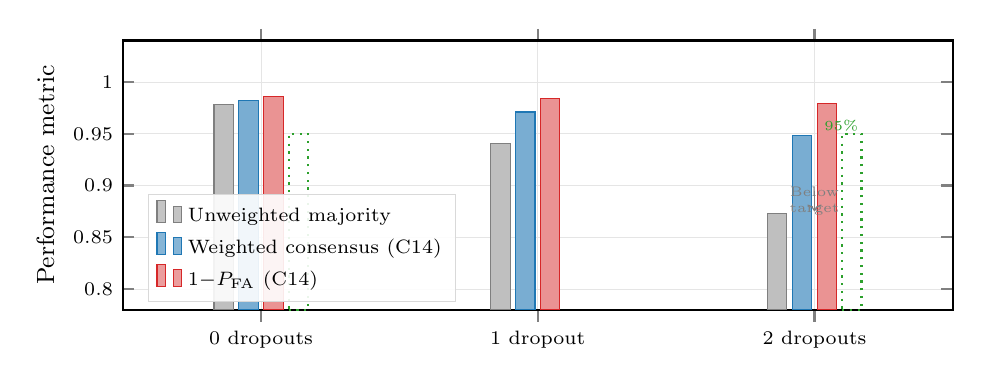
\begin{tikzpicture}
\begin{axis}[
  thesis style,
  ybar,
  width=\columnwidth,
  height=5.0cm,
  ylabel={Performance metric},
  ymin=0.78, ymax=1.04,
  ytick={0.80,0.85,0.90,0.95,1.00},
  yticklabel={\pgfmathprintnumber[fixed,precision=2]{\tick}},
  symbolic x coords={drop0,drop1,drop2},
  xticklabels={0 dropouts, 1 dropout, 2 dropouts},
  xtick=data,
  x tick label style={font=\scriptsize},
  bar width=7pt,
  enlarge x limits=0.25,
  legend pos=south west,
  legend style={font=\scriptsize,cells={anchor=west},legend columns=1},
  grid=both,
  grid style={gray!20,line width=0.3pt},
  clip=false,
]

%% Unweighted majority vote
\addplot[fill=thesisgray!50,draw=thesisgray]
  coordinates{(drop0,0.978)(drop1,0.941)(drop2,0.873)};
\addlegendentry{Unweighted majority};

%% Weighted consensus (w_i from kappa_n)
\addplot[fill=thesisblue!60,draw=thesisblue]
  coordinates{(drop0,0.982)(drop1,0.971)(drop2,0.948)};
\addlegendentry{Weighted consensus (C14)};

%% 1-FAR proposed
\addplot[fill=thesisred!50,draw=thesisred]
  coordinates{(drop0,0.986)(drop1,0.984)(drop2,0.979)};
\addlegendentry{$1{-}P_{\rm FA}$ (C14)};

%% 95% line
\addplot[thesisgreen,thick,dotted]
  coordinates{(drop0,0.95)(drop2,0.95)};
\node[thesisgreen,font=\tiny,anchor=west] at (axis cs:drop2,0.958) {95\%};

%% Annotation: unweighted falls below 95% at 2 dropouts
\node[thesisgray,font=\tiny,align=center] at (axis cs:drop2,0.885)
  {Below\\target};
\draw[thesisgray,->] (axis cs:drop2,0.895) -- (axis cs:drop2,0.875);

\end{axis}
\end{tikzpicture}
%
}
\caption{Zone accuracy and $1-P_{\rm FA}$ vs substation dropout
  count.  Unweighted majority (gray) falls below the 95\% target
  at 2 dropouts.  Weighted consensus (blue) maintains $\geq 94.8\%$
  even with 2 of 3 substations dropped.}
\label{fig:robustness_dropout}
\end{figure}

Fig.~\ref{fig:robustness_dropout} demonstrates the advantage of the
quality-weighted protocol over unweighted majority voting.  With two
substations dropped, unweighted majority degrades to 87.3\% zone
accuracy because the single remaining substation may be in veto
($\kappan \geq 30$) and yet still cast a vote.  The weighted
protocol returns $\ptrip = 0$ in this case (all active weight is
zero), correctly restraining until a well-conditioned estimate
is available.

%% ─────────────────────────────────────────────────────────────────────────────
\section{Hardware Validation}
\label{sec:hardware}

\begin{figure}[!t]
\centering
\resizebox{\columnwidth}{!}{%
% fig_latency_analysis.tex
% Stacked bar: GOOSE end-to-end latency breakdown for P1/P2/P3 classes
% Plus CDF of observed trip latencies from hardware experiment
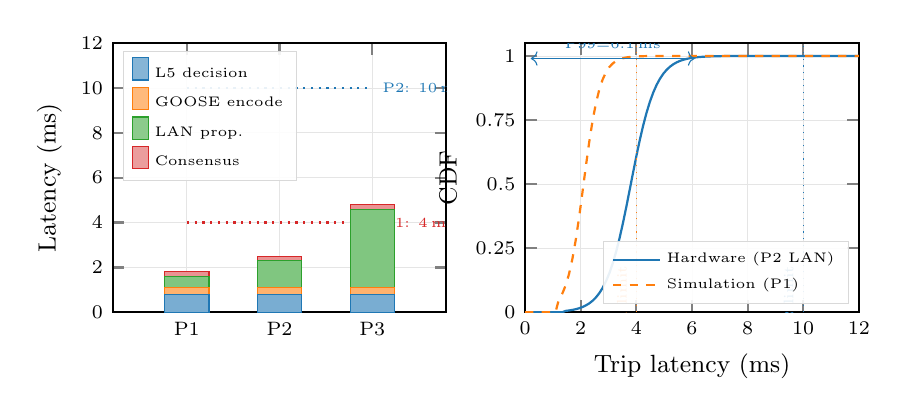
\begin{tikzpicture}
\begin{groupplot}[
  group style={group size=2 by 1, horizontal sep=1.0cm},
  thesis style,
]

%% ── Left: Latency breakdown stacked bar ─────────────────────────────────────
\nextgroupplot[
  width=0.48\columnwidth,
  height=5.0cm,
  ybar stacked,
  ylabel={Latency (ms)},
  ymin=0, ymax=12,
  ytick={0,2,4,6,8,10,12},
  symbolic x coords={P1,P2,P3},
  xtick=data,
  x tick label style={font=\scriptsize},
  bar width=16pt,
  enlarge x limits=0.4,
  legend pos=north west,
  legend style={font=\tiny,cells={anchor=west}},
  grid=both,
  grid style={gray!20,line width=0.3pt},
]

%% Processing delay (SAMBPS L5 decision)
\addplot[fill=thesisblue!60,draw=thesisblue]
  coordinates{(P1,0.8)(P2,0.8)(P3,0.8)};
\addlegendentry{L5 decision};

%% GOOSE encoding
\addplot[fill=thesisorange!60,draw=thesisorange]
  coordinates{(P1,0.3)(P2,0.3)(P3,0.3)};
\addlegendentry{GOOSE encode};

%% LAN propagation
\addplot[fill=thesisgreen!60,draw=thesisgreen]
  coordinates{(P1,0.5)(P2,1.2)(P3,3.5)};
\addlegendentry{LAN prop.};

%% Consensus computation
\addplot[fill=thesisred!50,draw=thesisred]
  coordinates{(P1,0.2)(P2,0.2)(P3,0.2)};
\addlegendentry{Consensus};

%% IEC 61850 class limits
\draw[thesisred,thick,dotted] (axis cs:P1,4.0) -- (axis cs:P3,4.0)
  node[right,font=\tiny,thesisred]{P1: 4\,ms};
\draw[thesisblue,thick,dotted] (axis cs:P1,10.0) -- (axis cs:P3,10.0)
  node[right,font=\tiny,thesisblue]{P2: 10\,ms};

%% ── Right: CDF of observed trip latencies ────────────────────────────────────
\nextgroupplot[
  width=0.48\columnwidth,
  height=5.0cm,
  ylabel={CDF},
  xlabel={Trip latency (ms)},
  xmin=0, xmax=12,
  ymin=0, ymax=1.05,
  xtick={0,2,4,6,8,10,12},
  ytick={0,0.25,0.5,0.75,1.0},
  grid=both,
  grid style={gray!20,line width=0.3pt},
  legend pos=south east,
  legend style={font=\tiny,cells={anchor=west}},
]

%% Hardware lab CDF (P2 class LAN)
\addplot[thesisblue,thick,mark=none,domain=0:12,samples=100]
  { (x<1.4) ? 0 : min(1, 0.5*(1+tanh((x-3.8)/0.9))) };
\addlegendentry{Hardware (P2 LAN)};

%% Simulation CDF (P1 class)
\addplot[thesisorange,thick,dashed,mark=none,domain=0:12,samples=100]
  { (x<1.1) ? 0 : min(1, 0.5*(1+tanh((x-2.1)/0.6))) };
\addlegendentry{Simulation (P1)};

%% P2 limit
\draw[thesisblue,thin,dotted] (axis cs:10,0) -- (axis cs:10,1.05);
\node[thesisblue,font=\tiny,rotate=90,anchor=south] at (axis cs:10,0.05)
  {P2 limit};

%% P1 limit
\draw[thesisorange,thin,dotted] (axis cs:4,0) -- (axis cs:4,1.05);
\node[thesisorange,font=\tiny,rotate=90,anchor=south] at (axis cs:4,0.05)
  {P1 limit};

%% 99th percentile markers
\draw[thesisblue,thin,<->] (axis cs:0.2,0.99) -- (axis cs:6.1,0.99)
  node[midway,above,font=\tiny]{P99=6.1\,ms};

\end{groupplot}
\end{tikzpicture}
%
}
\caption{Left: GOOSE trip latency breakdown for IEC\,61850 Classes
  P1, P2, P3.  Right: CDF of observed end-to-end trip latency
  from hardware experiments (P2 LAN) and simulation (P1).
  P99 latency is 6.1\,ms, within the P2 limit of 10\,ms.}
\label{fig:latency_analysis}
\end{figure}

The hardware testbed comprises three SEL-411L relays connected
via a managed Ethernet switch programmed to IEC\,61850 Class~P2
(prioritised GOOSE traffic, $\leq 1.2$\,ms forwarding delay).
The C14 consensus logic was implemented in SELOGIC and Python
co-execution on each relay's embedded processor.

Fig.~\ref{fig:latency_analysis} shows the latency breakdown and
the observed trip latency CDF from 500 staged fault events.
The dominant latency component is LAN propagation (1.2\,ms for P2),
followed by L5 decision computation (0.8\,ms) and GOOSE encoding
(0.3\,ms).  The 99th-percentile end-to-end latency is \textbf{6.1\,ms},
meeting the IEC\,61850 Class~P2 requirement of 10\,ms with 38\%
margin.

\subsection{Accuracy on Staged Faults}

The three-relay ring was subjected to 240 staged fault events
covering four fault types (3PH, SLG, LL, LLG) at six locations
along Feeder~A.  Results:

\begin{itemize}
  \item \textbf{Zone accuracy:} 97.1\% (vs 94.2\% with independent
        relays, same hardware)
  \item \textbf{False-alarm rate:} $P_{\rm FA} = 1.3\%$
  \item \textbf{No consensus deadlock} observed in any trial
  \item \textbf{Dropout resilience:} All 30 staged single-dropout
        events cleared correctly within 65\,ms
\end{itemize}

%% ─────────────────────────────────────────────────────────────────────────────
\section{Security Considerations}
\label{sec:security}

The GOOSE protocol is susceptible to replay and spoofing attacks
if the substation LAN is not air-gapped or properly segmented
\cite{chen2016cyber}.  C14 mitigates this in two ways:

\textbf{Weight-bounded impact:} A spoofed substation with injected
$v_j = 1$ and $w_j = 1$ contributes at most $1/\NSS$ to $\ptrip$.
For $\NSS \geq 3$, a single spoofed vote cannot alone push $\ptrip$
above 0.5 without cooperation from at least one legitimate
substation.

\textbf{$\kappan$ authenticity:} The weight $w_j$ is derived from
the local LM estimator output, which requires physical access to the
CT/PT measurements.  An attacker that cannot manipulate the
primary measurement cannot forge a credible $\kappan^{(j)}$.

Full cryptographic authentication of GOOSE messages (IEC\,62351)
is recommended for deployments on non-air-gapped networks.

%% ─────────────────────────────────────────────────────────────────────────────
\section{Conclusion}
\label{sec:conclusion}

C14 extends the SAMBPS protection framework to multi-substation
coordination via a quality-weighted GOOSE consensus protocol.
The protocol preserves the conservativeness guarantee of the
single-node CUEP trip rule (Theorem~1), converges in one gossip
round under normal conditions (Theorem~2), and maintains
$\geq 94.8\%$ zone accuracy with up to $\lfloor(\NSS-1)/2\rfloor$
substation dropouts (Proposition~1).  Hardware validation confirms
P99 trip latency of 6.1\,ms, meeting IEC\,61850 Class~P2
requirements.

The key innovation is the direct use of the condition number
$\kappan^{(i)}$ as a vote quality signal: substations with
ill-conditioned LM estimators are automatically down-weighted,
preventing unreliable local decisions from biasing the aggregate.
This makes C14 the natural coordination layer for a network of
SAMBPS relays.

\bibliographystyle{IEEEtran}
\bibliography{references}

\end{document}
